\section{Motor}

Nesta secção pretende-se descrever três pontos essenciais desta fase: as
estruturas de dados, algoritmos e processos de \emph{rendering}. Note-se que
o foco do \emph{rendering} será o uso de \emph{vertex array objects} por
oposição ao modo imediato de forma a obter uma maior eficiência.  


\subsection{\emph{Vertex Array Objects}}

O OpenGL possibilita dois modos de renderização: o modo imediato
e o \emph{vertex buffer objects} (VBOs). Os VBOs permitem um ganho substancial
de performance, uma vez que os dados são logo enviados para a memória da placa
gráfica onde residem, e por isso podem ser renderizados diretamente da placa
gráfica. O modo imediato usa a memória do sistema onde os dados são inseridos
\emph{frame} a \emph{frame}, usando uma API de renderização, o que causa peso
computacional sobre o processador.

Para a utilização das VBO's é necessário recorrer a criação de \emph{arrays} com os
dados para renderizar geometria. Com efeito, é necessário, em primeiro lugar,
ativar os \emph{arrays} com os diferentes tipos de dados e colocar os dados num
\emph{buffer object}. Estes \emph{arrays} são acedidos pelo seu endereço individual da
sua localização em memória, sendo então desenhadas as figuras geométricas dos
respetivos conteúdos dos \emph{arrays}.

Note-se que, no OpenGl, qualquer inteiro sem sinal pode ser usado como um
identificador de \emph{buffer objecto}. Estes identificadores podem-se
armazenados numa estrutura, sendo necessário, em seguida, gerar \emph{buffers} para os
vértices (um \emph{buffer} para cada \emph{array} com vértices ---
\texttt{glGenBuffers}) e ativar cada \emph{buffer} pelo seu identificador
(\texttt{glBindBuffer}) e preencher o \emph{buffer} com os dados de cada
\emph{array} de vértices previamente mencionados.

Para desenhar, a figura geométrica é necessário definir a semântica, ou seja,
definir o \emph{offset} relativo ao inicio do buffer (\texttt{glVertexPoint}),
consoante o tipo de dados, fazer o bind do objecto apropriado para fazer
a renderização e renderizar os arrays de vertices usando a função adequada
(\texttt{glDrawArrays} ou \texttt{glDrawElements}).

Para utilizar a tecnologia dos VBO's criou-se uma estrutura \texttt{Models}, que
para além de ser composta por um apontador para a raiz da árvore
\emph{n-ária} que será mencionada na próxima secção, possui um vetor de
\texttt{GLuint} para armazenar os identificadores e uma tabela com os nomes dos
ficheiros com os vértices para a geometria associadas a um tipo \texttt{VBO},
que é constituído pelo número de vértices do \emph{vertex array} e o índice do
\emph{vertex array} no vetor de identificadores.  

Para utilizar os VBO's, como descrito acima inicializou-se \emph{buffer}  com função
\texttt{initBuffers}, após da leitura do ficheiro de vértices,  ativando-o,
gerando um \emph{buffer} para um identificador, fazendo o \emph{bind} de
seguida e preenchendo o \emph{buffer} com os dados.   

Para renderizar os VBO's criou-se a função \texttt{drawVBO}, que faz
o \emph{bind} do \emph{buffer} pelo índice do \emph{buffer} no tipo
\texttt{VBO}, define a semântica, com o tamanho no tipo \texttt{VBO}.
A função \texttt{drawElement}, procura um nome de ficheiro na tabela mencionada
acima, e caso exista, aplica a função \texttt{drawVBO}.


\subsection{Estruturas de Dados para Transformações}
\label{subsec:sec2}

Como a estrutura do ficheiro XML é uma árvore \emph{n-ária} escolheu-se uma
estrutura que se seguiu a mesma lógica. Assim construiu-se um tipo de dados,
a partir de um \emph{struct} com vários campos para guardar os valores de cada
grupo, onde se encontra um vetor de apontadores para outras estruturas deste
tipo \texttt{Group}, como se pode ver na \emph{Figura~\ref{fig:ssec2:strut}}.
Além do mais, a estrutura base possui um vetor de \emph{strings} para guardar
os nomes de modelos que se encontrarem descritos no ficheiro XML.\ Existe também,
um outro vetor para guardar apontadores de objetos do tipo
\texttt{Transformation}, que representa de forma genérica qualquer transformação
geométrica.

\begin{center} 	
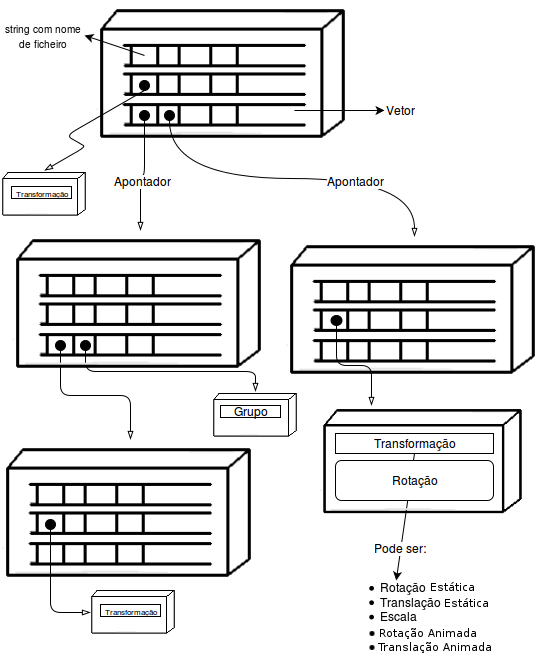
\includegraphics[width=\textwidth,height=\textheight,keepaspectratio]{resources/estrutura.png}
\captionsetup{type=figure, width=0.8\linewidth}
\caption{Árvore \emph{n-ária} para armazenamento de grupos}
\label{fig:ssec2:strut} 
\end{center}

Para a representação genérica de qualquer transformação geométrica, criou-se uma
estrutura de classes, onde a classe \texttt{Transformation} funciona como
superclasse abstrata, com cinco subclasses: \texttt{Rotation},
\texttt{Translation}, \texttt{Scale}, \texttt{AnimatedTranslation}
e \texttt{AnimatedRotation}. A superclasse possui um método virtual para
aplicação da transformação (\texttt{applyTrasformation}), que é aplicado no
contexto das suas subclasses quando invocado diretamente, ou como parte da
estrutura da hierarquia, à custa do polimorfismo que a linguagem de programação
C++ permite. Esta hierarquia pode ser vista com mais detalhe na
\emph{Figura~\ref{fig:ssec2:class}}. Parte da estrutura de classes é a classe
\texttt{Point3d} que representa um triplo de \texttt{floats} para as
coordenadas geométricas de um ponto em 3 dimensões. Adicionalmente a classe
implementa alguns métodos para cálculos de pontos e vetores, embora
o significado seja diferente entre estes dois conceitos. Algumas classes
implementam vetores deste tipo.

Posteriormente as classes \texttt{AnimatedTranslation}
e \texttt{AnimatedRotation} serão descritas com maior detalhe.



\begin{center} 	
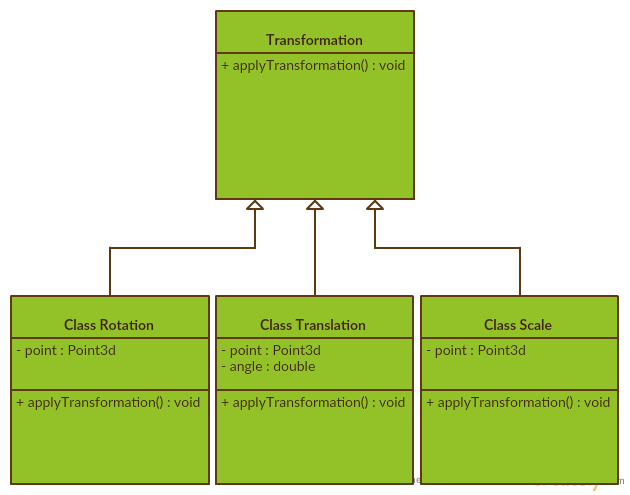
\includegraphics[width=\textwidth,height=\textheight,keepaspectratio]{resources/classes.png}
\captionsetup{type=figure, width=0.8\linewidth}
\caption{Hieraquia de classes de transformações geométricas}
\label{fig:ssec2:class} 
\end{center}


\subsection{Descrição do processo de leitura}

A função principal de leitura é a que está demonstrada no
\emph{Algoritmo~\ref{alg:ssec2:leitura}} e representa parte do processo de
leitura, no entanto decidiu-se remover partes acessórias de inicialização de
estruturas e afins. Esta função serve-se da estrutura de apontadores da árvore
que compõem a estrutura do documento XML para navegar na estrutura
recursivamente. 

Para além do apontador para o estrutura XML, passou-se por parâmetro um
apontador para a estrutura \texttt{Models}, que contem um apontador para a raiz
da árvore \emph{n-ária} e uma tabela (ou mapa) com os valores dos instâncias do
tipo \texttt{VBO}  para \emph{rendering} com o nome do ficheiro associado
(chave).Note-se que as estruturas em que se guardam valores dos elementos fazem
todas parte de um \texttt{Group}, tanto como o vetor de \emph{strings} com
o valor dos ficheiro, bem como o vetor de transformações e outros \texttt{Group}
no vetor de grupo, o seu acesso é por uma apontador para \texttt{Group}, exceto
os pares chave/valor guardados numa tabela na estrutura \texttt{Modelos}, com
o acesso feito a estrutura por apontador para a mesma.  

\begin{algorithm}

\caption{Função Principal Leitura}
\label{alg:ssec2:leitura} 
\footnotesize %% Smaller font size.
\begin{algorithmic}[1]
\Procedure{readXMLFromRootElement}{$XMLElement * elem$, $Modelos * models$,
$Group * grupo$}

\If{$elem = NULL$} 

\Return{}

\EndIf{}

\ForAll{$elem \in SIBLINGS$} 

\If{$elem = TRANSLATION \lor elems = SCALE$} 



\If{$elem = TRANSLATION$} 


\If{$elem = Attribute(TIME)$} 

\Comment{Obter o atributo $time$ e os valor dos pontos de controlo para animação
da translação}
\Comment{os atributos $x$, $y$, $z$ são alternativos.Se aparecerem é lhes
atribuído um valor. Caso contrário ficam com o valor $0$}

\State{\texttt{Guardar $x$, $y$, $z$ numa transformação como translação animada
com órbita}} 
 
\Else{} 
  

\Comment{os atributos $x$, $y$, $z$ são alternativos.Se aparecerem é lhes
atribuído um valor. Caso contrário ficam com o valor $0$}

\State{\texttt{Guardar $x$, $y$, $z$ numa transformação como translação}} 

\EndIf{}
 
\Else{} 

\State{\texttt{Guardar $x$, $y$, $z$ numa transformação como escala}} 
  
\EndIf{}

\ElsIf{$elem = ROTATION$} 


\If{$elem = Attribute(TIME)$} 

\Comment{Obter o atributo $time$ e os atributos $axis_{x, y, z}$. Para estes
últimos, se aparecerem é lhes atribuído um valor. Caso contrário ficam com o valor $0$}


\Comment{os atributos $x$, $y$, $z$ são alternativos.Se aparecerem é lhes
atribuído um valor. Caso contrário ficam com o valor $0$}
\State{\texttt{Guardar $x$, $y$, $z$ numa transformação como rotação animada}} 
 
\Else{} 

\Comment{os atributos $axis_{x, y, z}$ e $angle$ são alternativos. Se aparecerem
é lhes atribuído um valor. Caso contrário ficam com o valor $0$}

\EndIf{}
\State{\texttt{Guardar $axis_{x, y, z}$ e $angle$ numa transformação como
rotação}}

\ElsIf{$elem = MODELS$} 
 
\ForAll{$model \in MODELS$} 

\State{\texttt{Guardar atributo $file$ no vetor de vector<\emph{string}>
apontado por $grupo$}} 

\State{\texttt{Carregar lista de triângulos num $map$ associado a $file$,
apontados por $models$}}

\EndFor{}

\ElsIf{$elem = GROUP$} 

\State{\texttt{Criar novo $* novo\_grupo$}}

\State{\Call{readXMLFromRootElement}{$elem$, $novo\_grupo$}} 
 
\EndIf{}

\EndFor{}

\EndProcedure{}

\end{algorithmic}
\end{algorithm}

Como se pode ver no \emph{Algoritmo~\ref{alg:ssec2:leitura}}, as primeira
instruções referem-se ao caso de paragem da função recursiva que verifica se
o apontador do elemento, representa é um apontador não nulo. Em caso de nulo,
a função retorna para o sítio de onde foi invocada. 
Em seguida itera-se cada elemento que esteja no mesmo nível da árvore do
documento XML.\ podendo o elemento representar uma rotação, uma escala, uma
translação, um modelos ou grupos de modelos, e por fim um grupo.

Com efeito, se o elemento encontrado representar uma escala ou uma
translação caso for um translação e encontrar um atributo \texttt{time}, lê
o valor nesse atributo e itera pelos elementos \texttt{point}, verificando os
atributos x, y e z de cada ponto adicionando ao vetor de pontos da translação
animada (\texttt{AnimatedTranslation}) e adiciona a transformação ao vetor de
transformações. Caso contráriovobtêm-se os atributos \emph{x}, \emph{y} e \emph{z} e cria-se um
apontador, alocando memória para um instância da classe \texttt{Translation}
conforme a sua existência.
Caso for uma rotação e encontrar um atributo \texttt{time}, lê
o valor nesse atributo e os os valores \emph{axisX}, \emph{axisY}
e \emph{axisZ}, e guarda uma \texttt{AnimatedRotation}.Caso contrário
cria um  \texttt{Rotation} com \emph{axisX}, \emph{axisY}, \emph{axisZ}
e \emph{angle}, conforme a sua existência. Em ambos os casos a transformação
é adicionada ao vetor de transformações.


Se o elemento representar um conjunto de modelos, é efetuada uma navegação por
apontador para todos os elementos desse conjunto, obtendo o valor do atributo
\emph{file}. Este é guardado no vetor de vetor de \emph{strings} de
\texttt{Group}. De igual modo, através do valor do ficheiro é feita uma leitura
do mesmo, que tem os valores dos pontos dos vértices dos triângulos para
\emph{rendering}. Note-se que cada linha do ficheiro representa um vértice,
dado que cada linha tem os valores dos vértices separados por espaço,
e cada vértice tem as coordenadas \emph{x}, \emph{y} e \emph{z}. 

Por último, caso seja encontrado um elemento grupo, podem ocorrer uma de duas
situações: se o grupo está ao mesmo nível do grupo que antecedeu, ou seja é um
elemento \emph{irmão} ou se está dentro de um grupo, isto é, é um \emph{filhos}
do grupo anterior. No entanto, note-se que não existe uma verificação dos dois
caso no algoritmo, sendo efetuada uma chamada recursiva, com um novo elemento
grupo. Para ilustrar o caso, atente-se na
\emph{Figura~\ref{fig:ssec2:recleitura}}. A primeira invocação deste função,
representada pelo algoritmo, é precedida pela inicialização de um
\texttt{Group}, sendo este passado como parâmetro para esta função. Ou seja
é a raiz da árvore de \texttt{Group} e não possui quaisquer valores. O primeiro
elemento que a função encontra é um grupo, como se pode ver na figura, logo tem
que ser inicializado e adicionado à raiz, e apontador deste novo \texttt{Group}
é passado por parâmetro para a chamada recursiva da função. Dentro da chamada
recursiva, vão sendo adicionadas as transformações e modelos e se houver um novo
grupo, o processo repete-se. Algo de salientar é que a raiz, não tem
transformações nem modelos nos respetivos, nunca, e apenas o vetor com os
apontadores para os filhos é que é preenchido. Dado que um elemento com
a \emph{tag} \texttt{scene} pode apenas ter grupos e não transformações, assim
se justifica a raiz não ter transformações. Para o caso da
\emph{Figura~\ref{fig:ssec2:recleitura}}, a raiz terá apenas um \emph{filho},
que será o \emph{pai} de todos os outros grupos.   

À medida que vão sendo encontrados elementos XML nulos, ou seja, que não há mais
nada no mesmo nível, a função ainda entra na chamada recursiva, mas logo
retorna. Para clarificar, o \texttt{Group} para qual foi criada memória, logo
antes desta chamada recursiva tem de existir e é uma folha. Além do mais, como
demonstra a figura, as sucessivas chamadas recursivas vão retornando e voltando
para o sítio onde forma invocadas. Nesta chamadas recursivas, como o apontador
para o \texttt{Group} pai permanece localmente nessa função, vão sendo
adicionados novos os \emph{irmãos}. 

\begin{center}
\includegraphics[scale=0.75,keepaspectratio]{resources/exampleXML.png}
\captionsetup{type=figure, width=0.8\linewidth}
\caption{Diagrama representativo da recursividade do processo de leitura}
\label{fig:ssec2:recleitura} 
\end{center}


\newpage
\subsection{Descrição do ciclo de \emph{rendering}}



Para fazer o \emph{rendering} da estrutura de dados em memória, implementou-se
uma função de travessia da árvore, colocada na função \texttt{renderScene}, após
a função \texttt{glLoadIndentity} e \texttt{gluLookAt}, nesta sequência.
O \emph{Algoritmo~\ref{alg:ssec2:traverse}} representa a função que efetua esta
travessia.

Com efeito, a primeira instrução é a \texttt{glPushMatrix}, uma vez que se
pretende colocar uma matriz para aplicação das transformações no topo da
\emph{stack} de matrizes do \emph{OpenGL}. Em seguida, para cada transformação
contida num \texttt{Group}, é invocada a função \texttt{applyTrasformation}, já
mencionada na \emph{Secção~\ref{subsec:sec2}}, que aplica as transformações
conforme o contexto, como já foi explicado.

Em seguida, é invocada a função \texttt{drawElement}, descrita no
\emph{Algoritmo~\ref{alg:ssec2:rendering}}. Esta função especifica a primitiva
para que será criada com os vértices em memória, neste caso com um triplo de
vértices. 


Os vértices estão contidos, em objetos do tipo \texttt{Triangle} que
por sua vez, contêm objetos do tipo \texttt{Point3d} com as coordenadas de cada
vértice. Para obter estes vértices e criar a primitiva com \texttt{glVertex3f},
é necessário obtêm todas as \emph{strings} com o nome dos ficheiros no vetor de
\emph{string} de cada \texttt{Group}. Como cada nome, procura-se pelo
nome de ficheiro na tabela a partir do apontador para \texttt{Modelos}. Se
a entrada existir, obtêm-se todos valores de \texttt{Triangle}, respetivos
vértices e coordenadas.

No seguimento desta instrução existe um ciclo para aceder a elementos do vetor
de apontadores pelo índice para \texttt{Group}. Cada elemento (apontador para
\texttt{Group}) em determinada posição do \emph{array} é passado por argumento
para a chamada recursiva da função. Quando o chamada recursiva retorna, o índice
é incrementado e o processo repete-se.\ A função termina quando não houver mais
elementos no vetor.  Ou seja, o índice é incrementando à medida que
a chamadas recursivas entram na memória automática (\emph{stack}) e retornam,
saindo da \emph{stack}. 

Por último, note-se que a \texttt{glPopMatrix} é executada logo após o retorno
da chamada recursiva. Uma vez que as transformações sejam herdadas é necessário
colocar matrizes na \emph{stack} de matrizes do \emph{OpenGL}, conforme se vai
descendo na árvore. Quando a função faz o \emph{pop} à \emph{stack} de matrizes,
faz-lo na mesma chamada recursiva da função.

\newpage

\begin{algorithm}
\caption{Função de travessia da árvore de \texttt{Group}}
\label{alg:ssec2:traverse} 
\footnotesize %% Smaller font size.
\begin{algorithmic}[1]

\Procedure{traverseTree}{$Modelos * models$, $Group *grupo$}

\State{\Call{glPushMatrix}{$~$}} 

\ForAll{$transformation \in grupo \to TRANSFORMATIONS$} 
 
\State{$transformation\to \Call{applyTransformation}{ }$} 
 
\EndFor{}

\State{\Call{drawElement}{$models$, $grupo$}} 

\State{$i \gets 0$} 

\While{$i < $ tamanho do \emph{array} $grupo \to FILHOS$}

\State{\Call{traverseTree}{$models$, $grupo\to FILHOS_{i}$}} 

\State{\Call{glPopMatrix}{$~$}} 

\State{$i \gets i = i + 1$}

\EndWhile{}

\EndProcedure{}

\end{algorithmic}
\end{algorithm}
%%%%%%%%%%%%%%%%%%%%%%%%%%%%%%%%%%%%%%%%%%%%%%%%%%%%%%%%%%

\subsection{Classe \texttt{AnimatedRotation}}

A classe \texttt{AnimatedRotation}, no método \texttt{applyTrasformation}
divide 360 graus pelo valor de \texttt{time} obtendo um $\Delta_{\text{grau}}$.
Em seguida é obtido o tempo global da aplicação com
\texttt{glutGet (GLUT\_ELAPSED\_TIME)}, sendo calculado um valor de $t$, através
do módulo do tempo global da aplicação, com a variável \texttt{time}*1000 (este
calculo é para apresentar o time nas mesma unidades do tempo global, ou seja
ms), sendo que o valor do módulo é divido por \texttt{time}*1000 para obter um
valor entre 0 e 1. O tempo global funciona como contador global, e quando
dividido pelo tempo da animação torna-se circular.

Para aplicar a animação de rotação basta multiplicar $t$ por 360 para obter um
valor entre 0 e 360.


\subsection{Classe \texttt{AnimatedTranslation}}

A classe \texttt{AnimatedTranslation} aplica o mesmo conceito do parâmetro
$t$ como descrito na secção anterior, para obter um valor entre 0 e 1. Note-se
que esta classe possui um vetor com os pontos de controlo para para curva cúbica
de \emph{Catmull-Rom}. Note-se que são no mínimo são 4 pontos, por que é o que
está na definição da curva, podendo ser mais, mas sempre iterando de 4 em
4 pontos (3 pontos anteriores mais um novo ponto do vetor).

O método \texttt{applyTrasformation} aplica a função
\texttt{renderCatmullRomCurve} e \texttt{getGlobalCatmullRomPoint} fazendo
a translação do ponto obtido desta.   

\paragraph{\emph{Splines} cúbicas \emph{Catmull-Rom}}

A curva cúbica \emph{Catmull-Rom} para dados pontos de controlo $P_{0}, P_{1},
P_{2} e P_{3}$, está definida de modo a que a tangente em cada ponto $P_{i}$
possa ser encontrada através da diferença entre os seus pontos vizinhos
$P_{i-1}$ e $P_{i+1}$

\begin{center}
 	
 	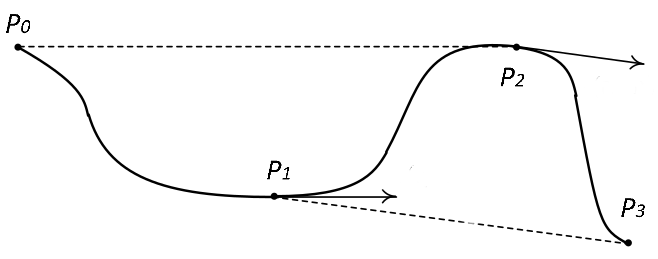
\includegraphics[scale=0.5,keepaspectratio]{resources/catmullDeriv.png}
 	\captionsetup{type=figure, width=0.8\linewidth}
	\caption{\emph{Spline} cúbica Catmull-Rom para os pontos $P_{0}, P_{1}, P_{2} e P_{3}$}
\label{fig:ssec1:diagram:plane:to:sphere} 
\end{center}

Esta curva pode ser escrita em forma de matriz:

\begin{gather*}
\frac{P_{2}-P_{0}}{2} = P_{1}^{'} = P^{'}(0) = c  \\
P_{1}                 = P(0)      = d        		  \\
P_{2}                 =P(1)       =a+b+c+d    		\\
\frac{P_{3}-P_{1}}{2} = P_{2}^{'} = P^{'}(1) = 3a+2b+c 
\end{gather*}


O que é equivalente a:

\begin{gather*}
P_{0} = a+b-c+d 		\\
P_{1} = P{0} = d 		\\
P_{2}=P(1)=a+b+c+d 	\\
P_{3}=6a+4b+2c+1
\end{gather*}

Este conjunto de equações pode-se representar na seguinte operação de matrizes:
\begin{equation}	
P=\begin{bmatrix}
		       P_{0} \\
		       P_{1} \\
		       P_{2} \\
		       P_{3}
		     \end{bmatrix}
= \begin{bmatrix}
 1 & 1 & -1 & 1 \\
 0 & 0 & 0 & 1 \\
 1 & 1 & 1 & 1 \\
 6 & 4 & 2 & 1
\end{bmatrix}
\begin{bmatrix}
a_{x} & a_{y} & a_{z}    \\
b_{x} & b_{y} & b_{z}    \\
c_{x} & c_{y} & c_{z}    \\
d_{x} & d_{y} & d_{z} 
\end{bmatrix} = C \times A
\label{eq:catmullmatrix}
\end{equation}
\begin{equation}
A = C^{-1}P
\label{eq:catmullmatrixa}
\end{equation}

Estes cálculos até agora demonstrados irão ser aplicados algoritmicamente no programa da seguinte maneira:
\begin{equation}	
\begin{bmatrix}
       x(u) & y(u) & z(u)             \\
\end{bmatrix} = 
\begin{bmatrix}
       t^{3} & t^{2} & t & 1          \\
\end{bmatrix}
\begin{bmatrix}
-0.5 & 1.5 & -1.5 & 0.5 \\
1 & -2.5 & 2 & -0.5     \\
-0.5 & 0 & 0.5 & 0      \\
0 & 1 & 0 & 0
\end{bmatrix}
\begin{bmatrix}
P_{0} \\
P_{1} \\
P_{2} \\
P_{3}
\end{bmatrix}
\label{eq:formula}
\end{equation}



\paragraph{\texttt{getGlobalCatmullRomPoint}}

Esta função aplica a fórmula da \emph{Equação~\ref{eq:formula}}, obtendo os
4 pontos de controlo, com os vetores com as coordenadas de forma similar ao
descrito nos \emph{patches} de Bézier  

\paragraph{\texttt{renderCatmullRomCurve}}

Itera de forma circular sobre os pontos armazenados no vetor de pontos com um
$t$ global obtendo todos os pontos da curva de Catmull-Rom




